\documentclass[pdftex]{beamer}
%\documentclass[notes=show]{beamer}
%\documentclass[xcolor=dvipsnames]{beamer}

\usepackage{amssymb}
\usepackage{latexsym}
\usepackage{amsfonts}
\usepackage{amsmath}
\usepackage[absolute,overlay]{textpos}
\usepackage[english]{babel}
\usepackage[latin1]{inputenc}
%\usepackage{times}
\usepackage[T1]{fontenc}
\usepackage{tabularx}
\newcolumntype{Y}{>{\small\raggedright\arraybackslash}X}
\usepackage{graphicx}
\usepackage{bigstrut}
\usepackage{bbm}
\usepackage{mathrsfs}
\usepackage{epsfig}
\usepackage{array}
\usepackage{xcolor}

\mode<presentation> {
%\usetheme[left,width=1.7cm]{Berkeley}
%\usetheme{default}
\usetheme{Boadilla}
  \usecolortheme[RGB={103,102,204}]{structure}
%\usecolortheme{dove}
  \useoutertheme{infolines}
  \setbeamercovered{transparent}
 }

%\renewcommand{\familydefault}{cmss}
%\renewcommand{\mathrm}{\mathsf}
%\renewcommand{\textrm}{\textsf}
\usefonttheme{serif}
\newcommand{\X}{{\mathbf{X}}}
\newcommand{\x}{{\mathbf{x}}}
\newcommand{\E}{\mathsf{E}}
\newcommand{\V}{\mathsf{Var}}


    %%%%%%%%%%%%%%%%%%%%%%%%%%%%%%%%%%%%%%%%%%%%%%%%%%%%%%%%%%%%%%%%%%%%%%%%%%%%%%
    %         Neue Kommandos f�r fette Mathebuchstaben innerhalb von Formeln     %
    %%%%%%%%%%%%%%%%%%%%%%%%%%%%%%%%%%%%%%%%%%%%%%%%%%%%%%%%%%%%%%%%%%%%%%%%%%%%%%
    \newcommand{\bom}{\boldmath}
    \newcommand{\ubom}{\unboldmath}
    \newcommand{\mb}{\mathbf}

    \newcommand{\fmalpha}{\mbox{\bom${\alpha}$}}               %Fettes alpha
    \newcommand{\fmbeta}{\mbox{\bom${\beta}$}}                 %Fettes beta
    \newcommand{\fmgamma}{\mbox{\bom${\gamma}$}}               %Fettes gamma
    \newcommand{\fmdelta}{\mbox{\bom${\delta}$}}               %Fettes delta
    \newcommand{\fmepsilon}{\mbox{\bom${\epsilon}$}}           %Fettes epsilon
    \newcommand{\fmvarepsilon}{\mbox{\bom${\varepsilon}$}}     %Fettes varepsilon
    \newcommand{\fmzeta}{\mbox{\bom${\zeta}$}}                 %Fettes zeta
    \newcommand{\fmeta}{\mbox{\bom${\eta}$}}                   %Fettes eta
    \newcommand{\fmta}{\mbox{\bom${\theta}$}}                  %Fettes theta (ta)
    \newcommand{\fmvarta}{\mbox{\bom${\vartheta}$}}         	 %Fettes vartheta (ta)
    \newcommand{\fmiota}{\mbox{\bom${\iota}$}}                 %Fettes iota
    \newcommand{\fmkappa}{\mbox{\bom${\kappa}$}}               %Fettes kappa
    \newcommand{\fmla}{\mbox{\bom${\la}$}}                     %Fettes lambda (la)
    \newcommand{\fmmu}{\mbox{\bom${\mu}$}}                     %Fettes mu
    \newcommand{\fmnu}{\mbox{\bom${\nu}$}}                     %Fettes nu
    \newcommand{\fmxi}{\mbox{\bom${\xi}$}}                     %Fettes xi
    \newcommand{\fmo}{\mbox{\bom${\o}$}}                       %Fettes o
    \newcommand{\fmpi}{\mbox{\bom${\pi}$}}                     %Fettes pi
    \newcommand{\fmvarpi}{\mbox{\bom${\varpi}$}}               %Fettes varpi
    \newcommand{\fmrho}{\mbox{\bom${\rho}$}}                   %Fettes rho
    \newcommand{\fmvarrho}{\mbox{\bom${\varrho}$}}             %Fettes varrho
    \newcommand{\fmsigma}{\mbox{\bom${\sigma}$}}               %Fettes sigma
    \newcommand{\fmvarsigma}{\mbox{\bom${\varsigma}$}}         %Fettes varsigma
    \newcommand{\fmtau}{\mbox{\bom${\tau}$}}                   %Fettes tau
    \newcommand{\fmupsilon}{\mbox{\bom${\upsilon}$}}           %Fettes upsilon
    \newcommand{\fmphi}{\mbox{\bom${\phi}$}}                   %Fettes phi
    \newcommand{\fmvarphi}{\mbox{\bom${\varphi}$}}             %Fettes varphi
    \newcommand{\fmchi}{\mbox{\bom${\chi}$}}                   %Fettes chi
    \newcommand{\fmpsi}{\mbox{\bom${\psi}$}}                   %Fettes psi
    \newcommand{\fmomega}{\mbox{\bom${\omega}$}}               %Fettes omega
    \newcommand{\fmimath}{\mbox{\bom${\imath}$}}               %Fettes imath


\setbeamercolor{bibliography entry title}{fg=black}
\setbeamercolor{bibliography entry author}{fg=black}
\setbeamercolor{subsection in toc}{fg=structure}
\setbeamercolor{palette primary}{bg=structure, fg=white}
%\setbeamercolor{palette secondary}{bg=structure, fg=black}
%\setbeamercolor{palette tertiary}{bg=structure, fg=black}
\setbeamercolor{caption name}{fg=black} \setbeamersize{text margin
left=.8cm} \setbeamersize{text margin right=1cm}
\hypersetup{linkbordercolor={1 0 0}} \setbeamertemplate{navigation
symbols}{} \setbeamertemplate{headline}[default]

\setbeamertemplate{enumerate items}[default]

\newcounter{transfct}
\newcounter{begbs}
\newcounter{endbs}
\title[Linear Regression]{Econometrics 2 (Part 1)}

\author[Lychagin  \& Mu\c co]{Sergey Lychagin}
\institute[CEU]{Central European University}
\date{Winter 2020}

\AtBeginSection[] {
  \begin{frame}<handout:0>
    \frametitle{TOC}
    \tableofcontents[currentsection]
  \end{frame}
}

%\AtBeginSubsection[] {
%  \begin{frame}<beamer>
%   \frametitle{Outline}
%    \tableofcontents[currentsection,currentsubsection]
%  \end{frame}
%}

%\beamerdefaultoverlayspecification{<+->}


\begin{document}

\frame{\titlepage}

\begin{frame}
\frametitle{Linear Regression and What It Estimates}
\begin{itemize}
\item The conditional expectation function (CEF)
\item CEF and regression
\item Regression and causality
\item The conditional independence assumption (CIA)
\item Omitted variables bias
\item Application: effect of computer use on wages
\end{itemize}
\end{frame}

\begin{frame}
\frametitle{Statistical Model}

$X_i, Y_i$   ... random variables

$x_i, y_i \;\;\;i=1,...n$ sample of random draws

\begin{itemize}
\item[1. Step] Describe the \emph{statistical} relationship between $X_i$ and $Y_i$
\item[2. Step] \emph{Econometric} interpretation of the relationship, causality
\end{itemize}
\end{frame}


\begin{frame}
\frametitle{Conditional Expectation Function}

$Y_i$   dependent variable

$X_i $  vector of covariates  $(K \times 1)$
\bigskip

$E\left[Y_i|X_i \right]$  expectation of $Y_i $ holding $X_i$ fixed
\bigskip

$X_i $  random variable

$E\left[Y_i|X_i \right]$ random function

\bigskip
Example: conditional expectation of earnings given the level of schooling
\end{frame}

\frame{ \frametitle{}
\begin{center}
\begin{figure}[t]
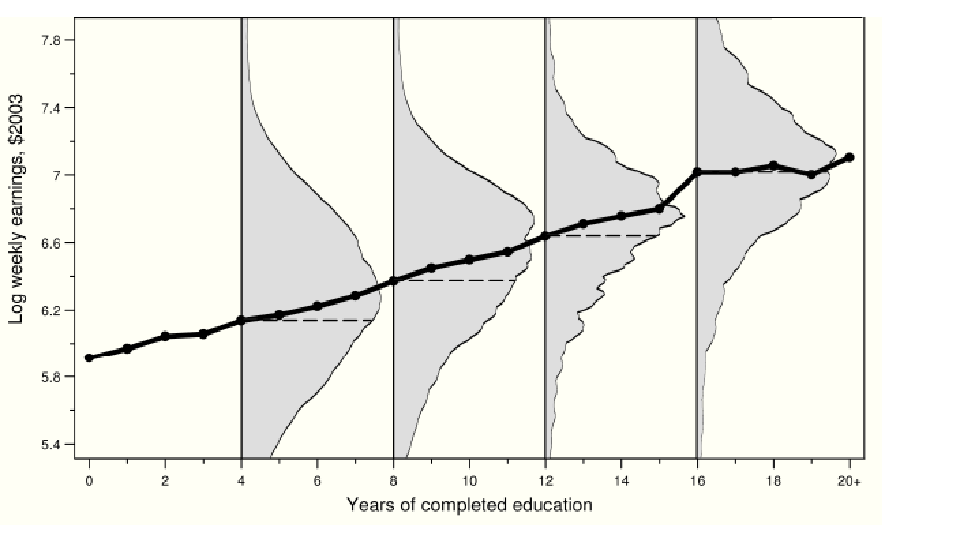
\includegraphics[width=1.1\linewidth]{graphs/cef.pdf}
\end{figure}
\end{center}
 }


\begin{frame}
\frametitle{CEF decomposition property}
\underline{Theorem}
\[ Y_i= E\left[Y_i|X_i \right] +\epsilon_i
\]
\begin{itemize}
\item[(i)] $\epsilon_i$ is mean independent of $X_i$, $E\left[\epsilon_i|X_i \right] =0$
\item[(ii)]  $\epsilon_i$ is uncorrelated with any function of $X_i$
\end{itemize}
\bigskip

The CEF breaks $Y_i$ into a part that is related to $X_i$ and one that is \emph{orthogonal} to $X_i$.
\end{frame}

\begin{frame}
\frametitle{Regression Function}

Best fitting line generated by minimizing the expected square errors
\[ \beta= \underset{b}{argmin}\;  E\left[(Y_i - X_i' b )^2 \right]
\]
%\bigskip

where $b $  is a   $(K \times 1)$ coefficient vector.
\bigskip

First order condition
\begin{eqnarray*}
&&E\left[X_i (Y_i - X_i' b ) \right] =0 \\
\beta &=& E\left[X_i  X_i' \right] ^{-1}E\left[X_i  Y_i \right]
\end{eqnarray*}
By construction the \emph{residual} $e_i=Y_i - X_i'\beta$ is uncorrelated with $X_i$
\end{frame}

\begin{frame}
\frametitle{Bivariate regression function}

Best fitting line generated by minimizing the expected square errors
\[ \beta= \underset{b}{argmin}\;  E\left[(Y_i - a - bX_i )^2 \right]
\]
%\bigskip

First order condition gives
\begin{eqnarray*}
\beta &=&\frac {Cov(Y_i , X_i)}{Var(X_i)} \\
\alpha &=& E\left[Y_i \right] - \beta E\left[X_i \right]
\end{eqnarray*}

%Estimator
%\begin{eqnarray*}
%\hat{\beta} &=&\frac {\sum(x_i -\bar{x})(y_i -\bar{y})}{\sum(x_i -\bar{x})^2} \\
%\hat{\alpha} &=& \bar{y} - \beta \bar{x}
%\end{eqnarray*}

\end{frame}

\begin{frame}
\frametitle{Multivariate regression function}

\[ Y_i= \beta_1 + \beta_2 x_{2i}+  ... + \beta_K x_{Ki} + e_i  \]

Regression Anatomy Formula
\begin{eqnarray*}
\beta_k &=& \frac {Cov(Y_i , \tilde{x}_{ik})}{Var(\tilde{x}_{ik})}
\end{eqnarray*}

where $\tilde{x}_{ik}$ is the residual from a regression of $x_{ki}$ on all other $X$ variables.

Proof
\begin{eqnarray*}
Cov(Y_i , \tilde{x}_{ik})&=& Cov(\beta_1 +  ... + \beta_K x_{Ki} + e_i , \tilde{x}_{ik}) \\
                                   &=& Cov(\ \beta_k x_{ki} , \tilde{x}_{ik}) = \beta_k Var(\tilde{x}_{ik})
\end{eqnarray*}

\end{frame}

\begin{frame}
\frametitle{Regression Function and CEF}
\underline{Theorem 1} (linear CEF theorem):

Suppose the CEF is linear, then the regression function is the CEF
\bigskip

\underline{Theorem 2} (regression CEF theorem):

$X_i' \beta$ provides the MMSE (minimum mean square error) linear approximation to $E\left[Y_i|X_i \right]$:
\[ \beta= \underset{b}{argmin}\;  E\left\{(E\left[Y_i|X_i \right] - X_i' b )^2 \right\}
\]
Even if the CEF is not linear, regression provides the best linear approximation.
\end{frame}

\frame{ \frametitle{}
\begin{center}
\begin{figure}[t]
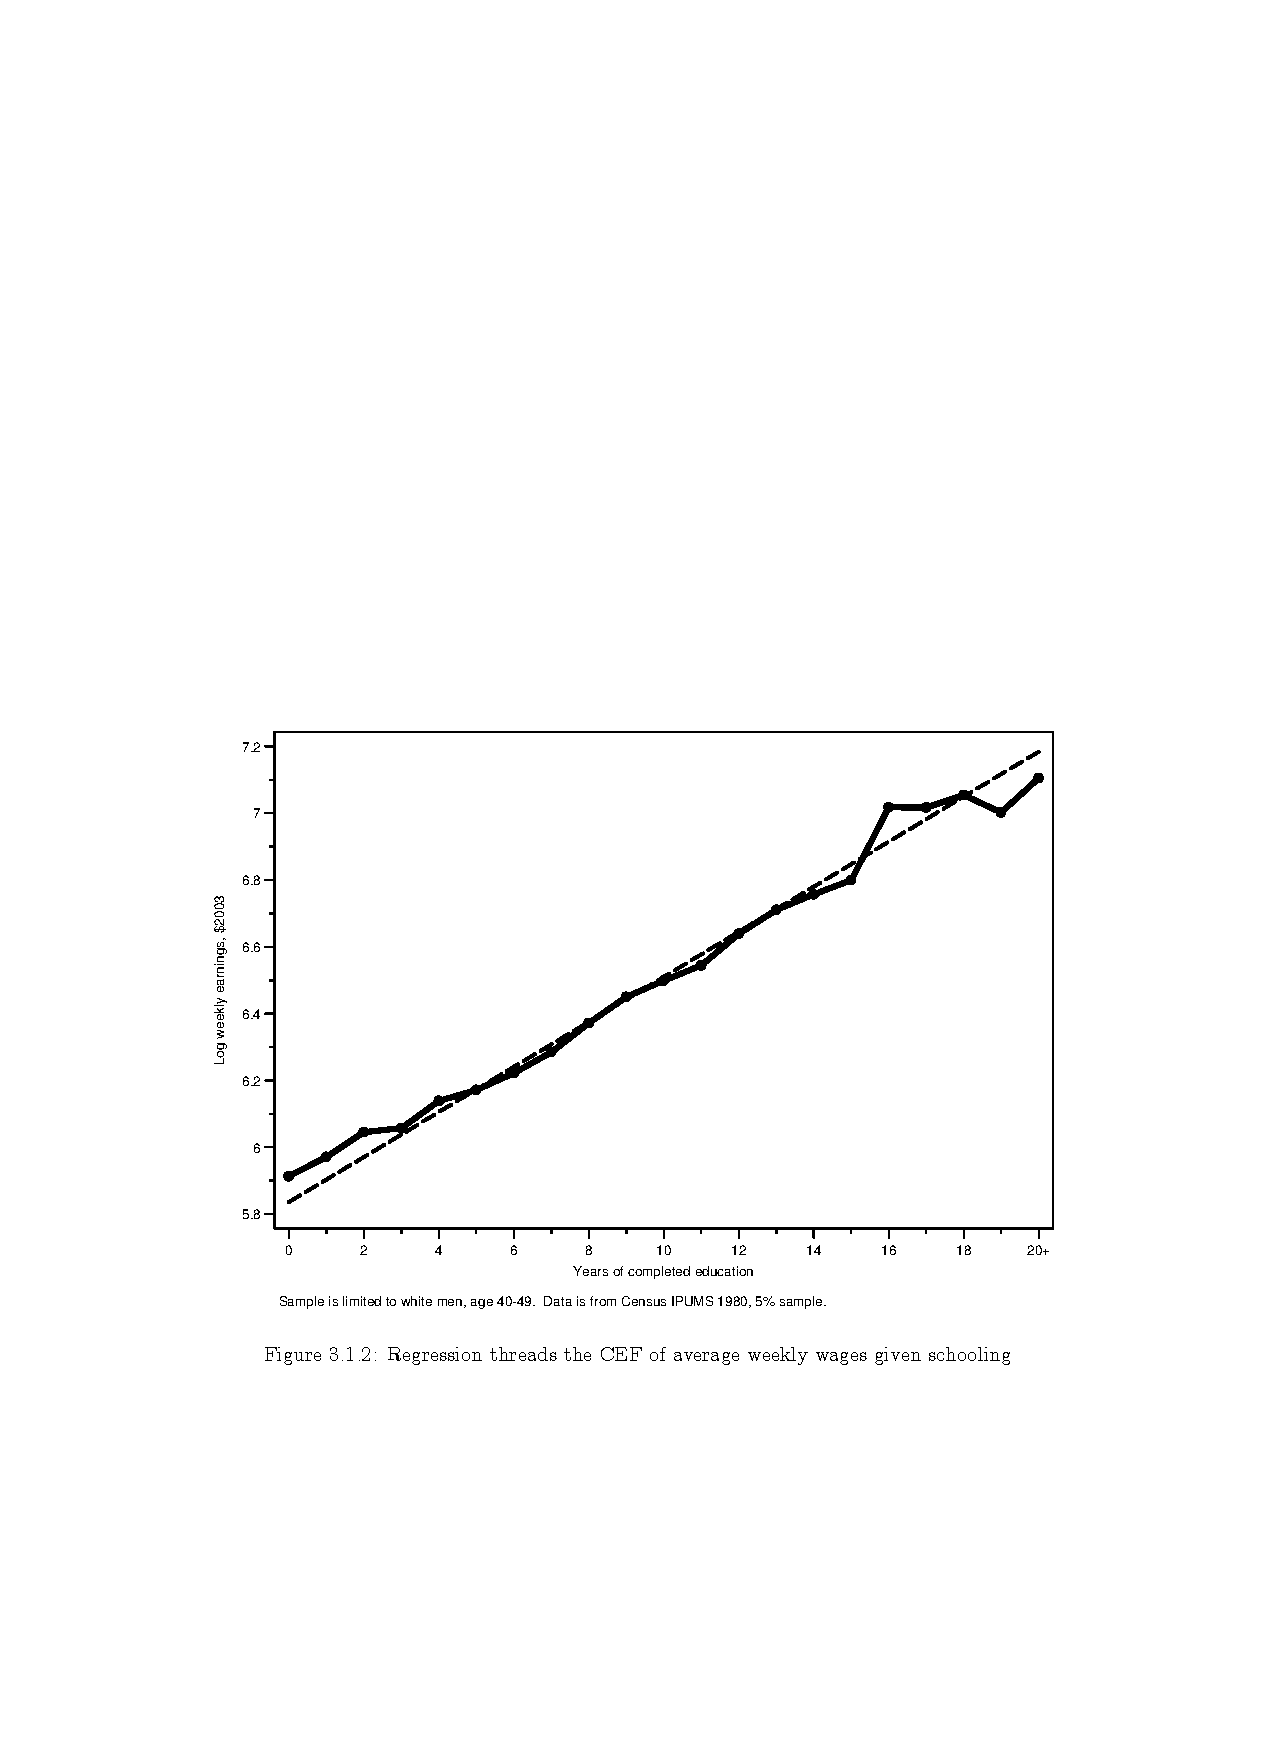
\includegraphics[width=1.1\linewidth]{graphs/regression_cef.pdf}
\end{figure}
\end{center}
 }


\begin{frame}{Estimation}
But we only observe a sample $\{x_i, y_i\}_{i=1,\dots,n}$, not the whole population. Approximate expectations with means $\Rightarrow$ OLS estimator:
\begin{equation*}
\beta = E\left[X_i  X_i' \right] ^{-1}E\left[X_i  Y_i \right]
\end{equation*}
turns into
\begin{equation*}
\widehat\beta = \left[\frac{1}{n}\sum_i x_i  x_i' \right] ^{-1}\left[\frac{1}{n}\sum_ix_i  y_i \right]
\end{equation*}
OLS is well-behaved: it is \emph{consistent} and \emph{asymptotically normal}:
\begin{itemize}
	\item $\widehat\beta\to \beta$ if $n\to\infty$
	\item $\sqrt{n}(\widehat\beta - \beta)\to N[0, V]$ if $n\to\infty$
\end{itemize}
\end{frame}

%%\end{document}
%
%\begin{frame}
%\frametitle{Saturated Models}
%\begin{itemize}
%\item Regression models with discrete explanatory variables, where the model includes a separate parameter for all possible values taken on by the explanatory variables.
%\end{itemize}
% Example 1:
%\[\begin{array}{cl}
%    y_{i} &\text{hourly wages} \\
%    s_{i} & \text{schooling, } s_{i}=0,1,...,\tau
%  \end{array}
%\]
%\begin{itemize}
%\item Saturated regression
%\begin{eqnarray*}
%	y_{i} &=& \alpha+\beta_{1}d_{1 i}+...+\beta_{\tau}d_{\tau i}+\epsilon_{i} \\
%  d_{ij} &=& 1\left[s_{i}=j\right]
%\end{eqnarray*}
%\end{itemize}
%\end{frame}
%
%
%
%\begin{frame}
%\frametitle{Saturated Models}
%\begin{itemize}
%\item Dummy variables are indicating each schooling level
%\item $\beta_{j}$ j-th level of schooling effect
%
%\[\begin{array}{cl}
%    \beta_{j}&= E\left[Y_{i}|s_{i}=j\right]-E\left[Y_{i}|s_{i}=0\right]\\
%   \alpha&= E\left[Y_{i}|s_{i}=0\right] \text{, }   s_{i}=0 \text{ (reference group)}
%    \end{array}
%\]
%
%\item One parameter for any possible $j$
%\item Saturated models perfectly fit the CEF
%
%(CEF is linear function of the set of dummy variables)
%\end{itemize}
%\end{frame}
%
%
%
%\begin{frame}
%\frametitle{Saturated Models}
%
%Example 2:
%
%\begin{itemize}
%\item Two explanatory variables: College graduate and Sex
%
%\[
%\begin{array}{cl}
%    y_{i}=\alpha+\beta_{1}coll+\beta_{2}fem+\beta_{3}coll \times female+ \epsilon_{i}
% \end{array}
%\]
%
%
%\item $\beta_{1}$ and $\beta_{2}$ main effects; $\beta_{3}$ interaction term.
%
%\item Other Parametrizations:
%\[
%\begin{array}{cl}
%    y_{i}=\tilde{\beta_{1}}male_{\_}coll+\tilde{\beta_{2}}male_{\_}nocoll+\tilde{\beta_{3}}female_{\_}coll\\
%     +\tilde{\beta_{4}} female_{\_}nocoll
%    \end{array}
%\]
%
%
%\item CEF has four possible values: $x_{1i}$ college and $x_{2i}$ female
%
%\[
%\begin{array}{cl}
%E\left[Y_{i}|x_{1i}=0, x_{2i}=0\right]= & \alpha\\
%E\left[Y_{i}|x_{1i}=1, x_{2i}=0\right]= & \alpha+\beta_{1}\\
%E\left[Y_{i}|x_{1i}=0, x_{2i}=1\right]= & \alpha+\beta_{2}\\
%E\left[Y_{i}|x_{1i}=1, x_{2i}=1\right]= & \alpha+\beta_{1}+\beta_{2}+\beta_{3}
% \end{array}
%\]
%\end{itemize}
%
%\end{frame}
%
%
%\begin{frame}
%\frametitle{Saturated Models}
%Example 3:
%
%\begin{itemize}
% \item Multivalued schooling and Sex
%  \[
%  \begin{array}{cl}
%    y_{i}= \alpha+\sum_{j=1}^{\tau} \beta_{j} d_{ij}+ \gamma x_{2i}+\sum_{j=1}^{\tau}  \delta_{j} \left( d_{ij}\times x_{2i} \right)+\epsilon_{i}
%    \end{array}
%    \]
%  \item CEF has $\left(\tau+1\right)\times 2$ values
%  \item Saturated Model exactly fits CEF
%  \item Increasingly restrictive model: omitting some interactions\\
% e.g: Return to schooling is same for men and women
% \item But often models do not make sense! e.g:
%\begin{eqnarray*}
%y_{i}= \alpha+ x_{2i}+ \sum \delta_{j}\left(d_{ji}\times x_{2i}\right)+ \epsilon_{i}
%\end{eqnarray*}
% different returns to schooling levels \emph{only} for women
%\end{itemize}
%\end{frame}
%



\begin{frame}
\frametitle{Causality}

\begin {itemize}



\item Interpretation of CEF, causal vs non-causal:
\begin{itemize}
	\item Non-causal: What is the average difference in earnings between people with $x+1$ and $x$ years of schooling?
		\item Causal: What would people earn, on average, if we give them 1 year of schooling holding \emph{all} other characteristics fixed?
\end{itemize}

\item Regression causal $\Leftrightarrow$ CEF causal
\item Causal Effect: difference in average \emph{potential outcome}
\item The CEF is causal if it describes differences in the average potential outcomes for a fixed reference group

\end{itemize}
\end{frame}


\begin{frame}
\frametitle{Conditional Independence Assumption (CIA)}

Idea:
\begin{itemize}
\item \emph{selection on observables}
\item Causal variable is independent of potential outcome conditional on observable variables $X$ (ability, family, etc.)
\item Intuitively, for all individuals with the same $X$, assignment to treatment is as good as random.
\end{itemize}
\end{frame}



\begin{frame}
\frametitle{Potential outcome framework}
\begin{eqnarray*}
c_i && \text{College} \\
Y_i &=& \left\{ \begin{array}{cc}
                                                Y_{1i} & \text{if}\;\; c_i=1 \\
                                                Y_{0i} & \text{otherwise}\;\;
                            \end{array} \right.\\
                        X_i&& \text{observable controls: family income, age, etc.}
\end{eqnarray*}
\begin{itemize}
\item Causal Effect $Y_{1i}-Y_{0i}$
\item We want to  estimate average $Y_{1i}-Y_{0i}$ for some group
\item e.g. $E\left[Y_{1i}-Y_{0i}| c_{i}=1\right ]$  average causal effect for those who went to college.
\item Remember:
\begin{eqnarray*}
E\left[Y_{i}|c_{i}=1\right]-E\left[Y_{i}|c_{i}=0\right]&=&E\left[Y_{1i}-Y_{0i}|c_{i}=1\right]\\
 &+&\underset{\text{selection bias}}{\underbrace{E\left[Y_{0i}|c_{i}=1\right]-E\left[Y_{0i}|c_{i}=0\right]}}
\end{eqnarray*}
\end{itemize}
\end {frame}


\begin{frame}
\frametitle{CIA}
The conditional independence assumption asserts that conditional on observable variables $X_{i}$ selection bias disappears:
\begin{eqnarray*}
\left\{Y_{0i}, Y_{1i}\right\} \amalg  c_{i}|X_{i}
\end{eqnarray*}
\begin{eqnarray*}
  \underbrace{E(Y_i|X_{i}, c_{i}=1)-E(Y_i|X_{i},c_{i}=0)}_{\text{observed difference |X}}=\underbrace{E(Y_{1i}-Y_{0i}|X_{i})}_{\text{difference in pot outcome |X}}
\end{eqnarray*}

\end{frame}



\begin{frame}
\frametitle{Multivalued Case}
Multivalued causal variable $s_i$:  level of schooling
\bigskip

Potential earnings for individual \emph{i} with \emph{s} years of schooling
\begin{eqnarray*}
Y_{s_i}= f_{i}\left(s\right)
\end{eqnarray*}
Conditional independence assumption:
\[ Y_{s_i}\amalg s_{i}| X_{i} \;\;\;\text{for all} \;\; s
\]
$s_i$ is \emph{as good as randomly assigned} conditional on $X_i$

Causal interpretation:
\begin{eqnarray*}
E\left[Y_{i}|X_{i}, s_{i}=s\right]-E\left[Y_{i}|X_{i}, s_{i}=s-1\right]= E\left[f_{i}\left(s\right)-f_{i}\left(s-1\right)|X_{i}\right]
\end{eqnarray*}
\end{frame}


%\end{document}

\begin{frame}
\frametitle{Causality}
\begin{itemize}
\item In the potential outcome framework we get a causal effect for every value of $X_i$
\item Average over  $X_i$ using iterated expectations
\begin{eqnarray*}
E\left\{E \left[Y_{i}|X_{i}, s_{i}=12 \right]-E \left[Y_{i}|X_{i}, s_{i}=11\right]\right\}\\
=E\left\{E\left[f_{i}(12) -f_{i}(11)|X_{i}\right]\right\}=E\left[f_{i}\left(12\right)-f_{i}\left(11\right)\right]
\end{eqnarray*}
\item We also get a separate causal effect for each pair of levels of $s_i$, e.g. $(11,12), (12,13), ....$
\item Use regression to \emph{summarize} the effects


\end{itemize}
\end{frame}



\begin{frame}
\frametitle{Regression}
\begin{itemize}
\item Assumption: $f_{i}\left(s\right)$ is linear in $s$ and the same for all $i$

\item We estimate a weighted average of individual specific $f_{i}\left(s\right)-f_{i}\left(s-1\right)$
\bigskip

\item Causal Model:

\[\begin{array}{cl}

   f_{i}\left(s\right)= \alpha+\rho s +\eta_{i}
    \end{array}
\]

linear same relationship for everybody.
\item $\eta_{i}$  error component: unobserved factors determining potential earnings
\item Plug in observed values

\[\begin{array}{cl}

   Y_{i}= \alpha+\rho s_i +\eta_{i}
    \end{array}
\]

\item Problem: $s_{i}$ may be correlated with potential outcomes $f_{i}\left(s\right)$ via $\eta_{i}$.

\end{itemize}

\end{frame}



\begin{frame}
\frametitle{Conditional Independence}

 Suppose CIA holds given $X_{i}$ and the CEF of $\eta_i$ is linear in $X_i$. Then,
\[\begin{array}{cl}

   \eta_{i} =X_{i}^{'}\gamma +v_{i}
    \end{array}
\]

where  $\gamma$ is a vector of population regression coefficients
\[E\left[\eta_{i}|X_{i}\right]= X_i^{'}\gamma \]
important: the residual $v_{i}$ is uncorrelated with $X_{i}$.

\begin{eqnarray*}
    E\left[f_{i}\left(s\right)|X_{i},s_{i}\right] =E\left[f_{i}\left(s\right)|X_{i}\right]
       &=& \alpha+\rho s_i+ E\left[\eta_{i}|X_{i}\right]\\
        &=&\alpha+\rho s_i+ X_{i}^{'}\gamma\\
\end{eqnarray*}

We get the linear causal model:

\begin{eqnarray*}
    Y_{i}=\alpha+\rho s_{i}+ X_{i}^{'}\gamma+ v_{i}
\end{eqnarray*}



\end{frame}


\begin{frame}
\frametitle{Regression}

Linear causal model:

\begin{eqnarray*}
    Y_{i}=\alpha+\rho s_{i}+ X_{i}^{'}\gamma+ v_{i}
\end{eqnarray*}
\begin{itemize}
\item $v_{i}$ is not correlated with $s_{i}$, or $X_{i}$. $\rho$ represents causal effect.\\

\item Key assumption: the observable variables $X_{i}$ are the only reason that $\eta_{i}$, or $s_{i}$ are correlated (or $f_{i}\left(s\right)$, and $s_{i}$)

\item Note: $\gamma$ is not causal in general!
\end{itemize}

\end{frame}



\begin{frame}
\frametitle{Omitted Variable Bias}

OVB formula describes relationship between regression models  with different sets of control variables.

\begin{itemize}
\item Short Regression:

\begin{eqnarray*}
    Y_{i}=\tilde{\alpha}+\tilde{\rho} s_{i}+ \eta_{i}
\end{eqnarray*}

\item Long Regression:

\begin{eqnarray*}
    Y_{i}=\alpha+\rho s_{i}+ A_{i}\gamma+e_{i}
\end{eqnarray*}

where $A_{i}$ represents ability, family background.

\item If CIA applies given $A_{i}$ then $\rho$ is the coefficient of the linear causal model.
\end{itemize}

\end{frame}



\begin{frame}
\frametitle{Omitted Variables Bias Formula}

\begin{eqnarray*}
\widehat{\tilde{\rho}}=\frac{Cov\left(Y_{i}, s_{i}\right)}{V\left(s_{i}\right)}=\rho+\gamma^{'}\delta_{As}
\end{eqnarray*}
where $\delta_{As}$ vector of coefficients from regressions of $A_{i}$ on $s_{i}$
\bigskip

coef from short regression = coef from long regression \emph{plus} effect of omitted variables $*$ regression coef of omitted on included variables

\begin{eqnarray*}
   \frac{Cov\left(Y_{i}, s_{i}\right)}{V\left(s_{i}\right)} &=& \frac{Cov\left(\alpha+\rho s_{i}+ A_{i}^{'}\gamma+e_{i}, s_{i}\right)}{V\left(s_{i}\right)}\\
    &=&\frac{\rho V\left(s_{i}\right)+\gamma Cov\left(A_{i}, s_{i}\right)}{V\left(s_{i}\right)}\\
    &=& \rho + \gamma\frac{Cov \left(A_{i}, s_{i}\right)}{V\left(s_{i}\right)}\\
\end{eqnarray*}



\end{frame}



\begin{frame}
\frametitle{Interpretation}
\begin{itemize}
\item  $\delta_{As}=0$, if $A_{i}$ and $s_{i}$ are uncorrelated
\item Consequences of omitting $A_{i}$\\
\end{itemize}

Sign of bias
\begin{center}
\begin{tabular}{ l| c r }
  \hline
   & $Cov(A_{i},s_{i})  >0$&$Cov(A_{i},s_{i})  <0 $\\ \hline
   $\gamma >0$ & \color{red}{positive} &  \color{red}{negative}  \\ 
   $\gamma<0$   & \color{red}{negative}  &  \color{red}{positive} \\ \hline
\end{tabular}
\end{center}
\end{frame}

\frame{ \frametitle{}
\begin{center}
\begin{figure}[t]
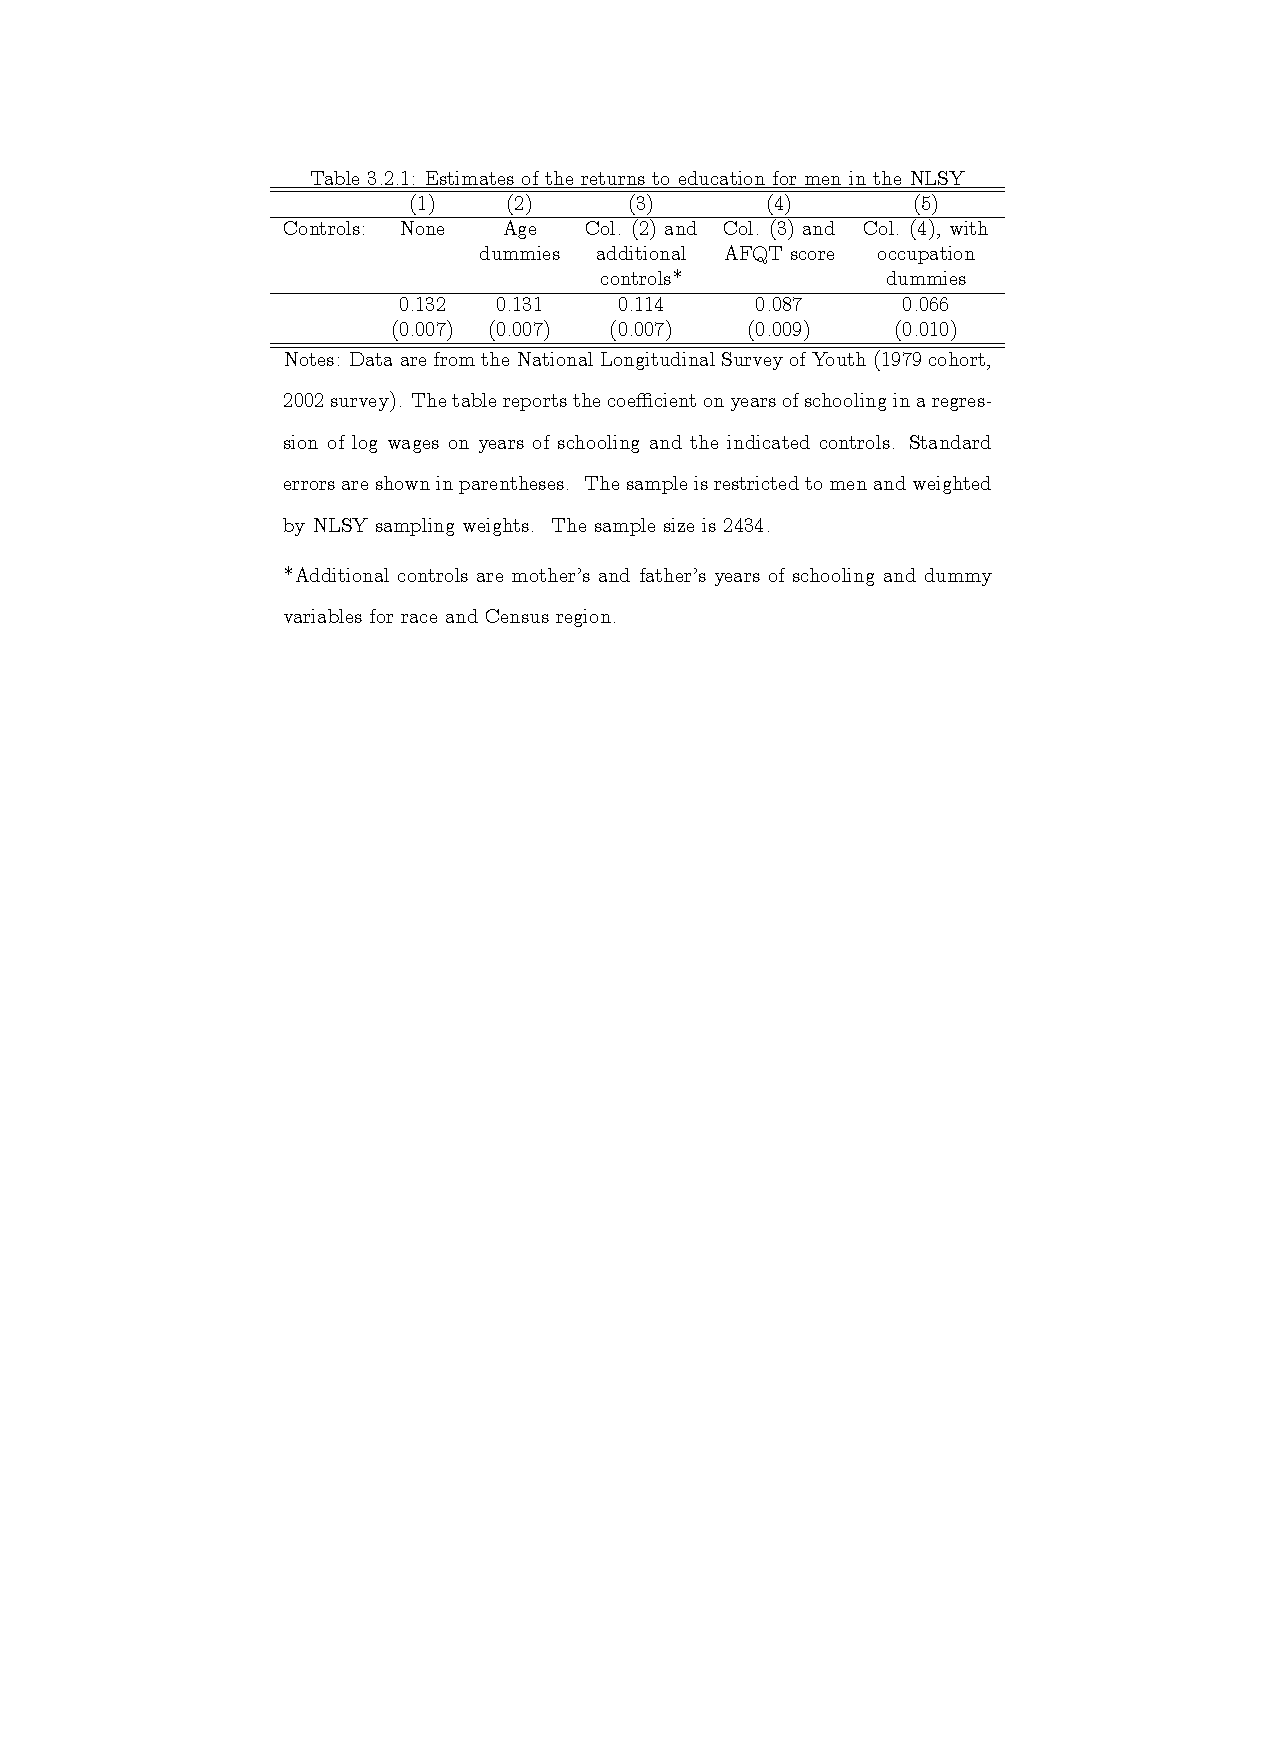
\includegraphics[width=0.9\linewidth]{graphs/ap_321.pdf}
\end{figure}
\end{center}
 }
 
 
 \begin{frame}{Bad Controls}
 \begin{itemize}
 	\item Control for covariates increases likelihood for a causal interpretation of the main relationship. Should we include any controls?
 	\item Caution:
 	\begin{itemize}
 		\item Bad controls-variables that might themselves be outcomes in the ``thought'' experiment.\\
 	\end{itemize}
 	
 	\item Example:
 	\begin{itemize}
 		\item Randomly assign college degree (causal effect of mean earnings) \\
 		\item Occupation correlated with earnings and education.\\
 	\end{itemize}
 	
 	\item Should we control for occupation? (white collar job)
 	
 \end{itemize}
 
\end{frame}

\begin{frame}{Bad Controls: more formally}
We relate earnings to the college education dummy. Control for occupation: use the white collar workers only ($W_i = 1$).
\begin{equation*}
Y_i = \alpha + \rho C_i + \epsilon_i, \quad\text{for all $i$ such that $W_i=1$}
\end{equation*}
Let's apply the potential outcome framework. What is the DGP?
\begin{enumerate}
\item Each agent is born with $(Y_{0i}, Y_{1i}, W_{0i}, W_{1i})$ -- wage and occupation for college/no-college state of the world.
\item Treatment is random (just for the sake of argument!)
\item If $C_i = 1$, then $Y_i=Y_{1i}$, $W_i=W_{1i}$ and vice versa.

\end{enumerate}
Key issue: occupation is an outcome. Selecting sample based on $W_i$ --- ``endogenous sample selection''.

\end{frame}

\begin{frame}
Interpret $\rho$ in the potential outcome framework:
\begin{align*}
\rho &= E[Y_i|C_i=1, W_i=1] - E[Y_i|C_i=0, W_i=1]\\
&= E[Y_{1i}|C_i=1, W_{1i}=1] - E[Y_{0i}|C_i=0, W_{0i}=1]\\
&= E[Y_{1i} - Y_{0i}|C_i=1, W_{1i}=1] \\
&\phantom{=} + E[Y_{0i}|C_i=1, W_{1i}=1] - E[Y_{0i}|C_i=0, W_{0i}=1]\\
&= \underbrace{E[Y_{1i} - Y_{0i}| W_{1i}=1]}_\text{effect for the ``white collar after college'' population} \\
&\phantom{=} + \underbrace{E[Y_{0i}|W_{1i}=1] - E[Y_{0i}| W_{0i}=1]}_\text{selection bias}
\end{align*}
Signing selection bias: need to know more on how agents decide on $W_i$. Casual intuition -- likely negative:
\begin{itemize}
\item $W_{0i}=1$ -- Mark Zuckerberg and Bill Gates
\item $W_{1i}=1$ -- median college graduate.
\end{itemize}
Note how the potential outcome model made the discussion tractable.
\end{frame}



\begin{frame}
\frametitle{Application: Returns to Computer Use}
\begin{itemize}
\item Alan B. Krueger, ``How Computers Have Changed the Wage Structure: Evidence from Microdata 1984 - 1989", QJE 1993
\item John E. DiNardo and Jorn-Steffen Pischke, ``The Returns to Computer Use Revisited: Have Pencils Changed the Wage Structure Too?", QJE 2004
\end{itemize}

\end{frame}


\begin{frame}
\frametitle{Returns to Computer Use: Motivation}

Facts:

   \begin{itemize}
     \item Returns to education rising over time.
     \item Potential explanation: Skill Biased Technological Change
     \item Empirical evidence: Returns to computer use
  \end{itemize}

Seminal study Krueger (1993)

\begin{itemize}
\item Cross sectional data on wages, computer on the job, CPS 1984, 1989
\item Causal effect of computer use on wages plus 15-20\% increase
\end{itemize}

Problem:
    \begin{itemize}
        \item Is there any unobservable characteristic $x^{*}$ correlated to computer use?
         So that all individuals with this characteristic would earn higher wages anyway?
\end{itemize}

\end{frame}

\frame{ \frametitle{}
\begin{center}
\begin{figure}[t]
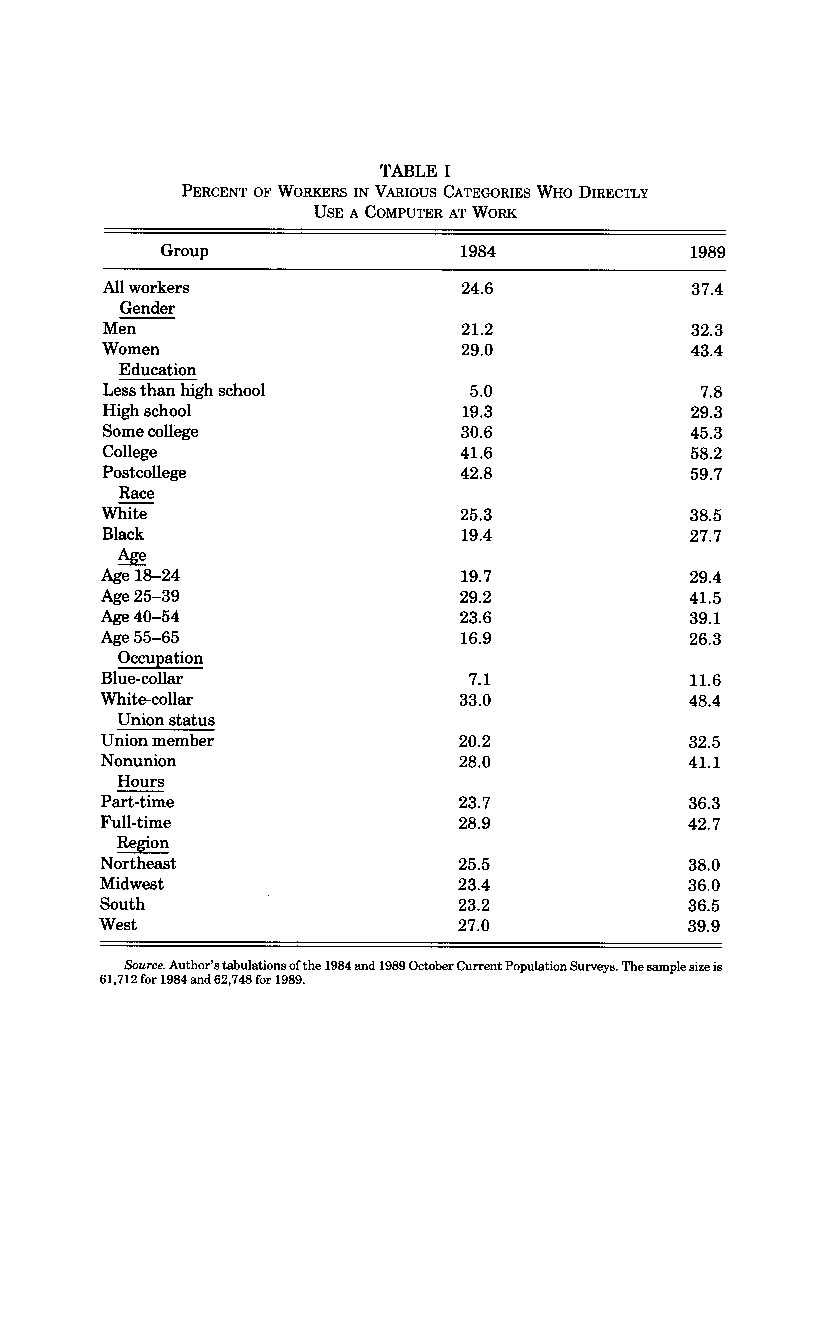
\includegraphics[width=0.7\linewidth]{graphs/kru_table1.pdf}
\end{figure}
\end{center}
 }

\frame{ \frametitle{}
\begin{center}
\begin{figure}[t]
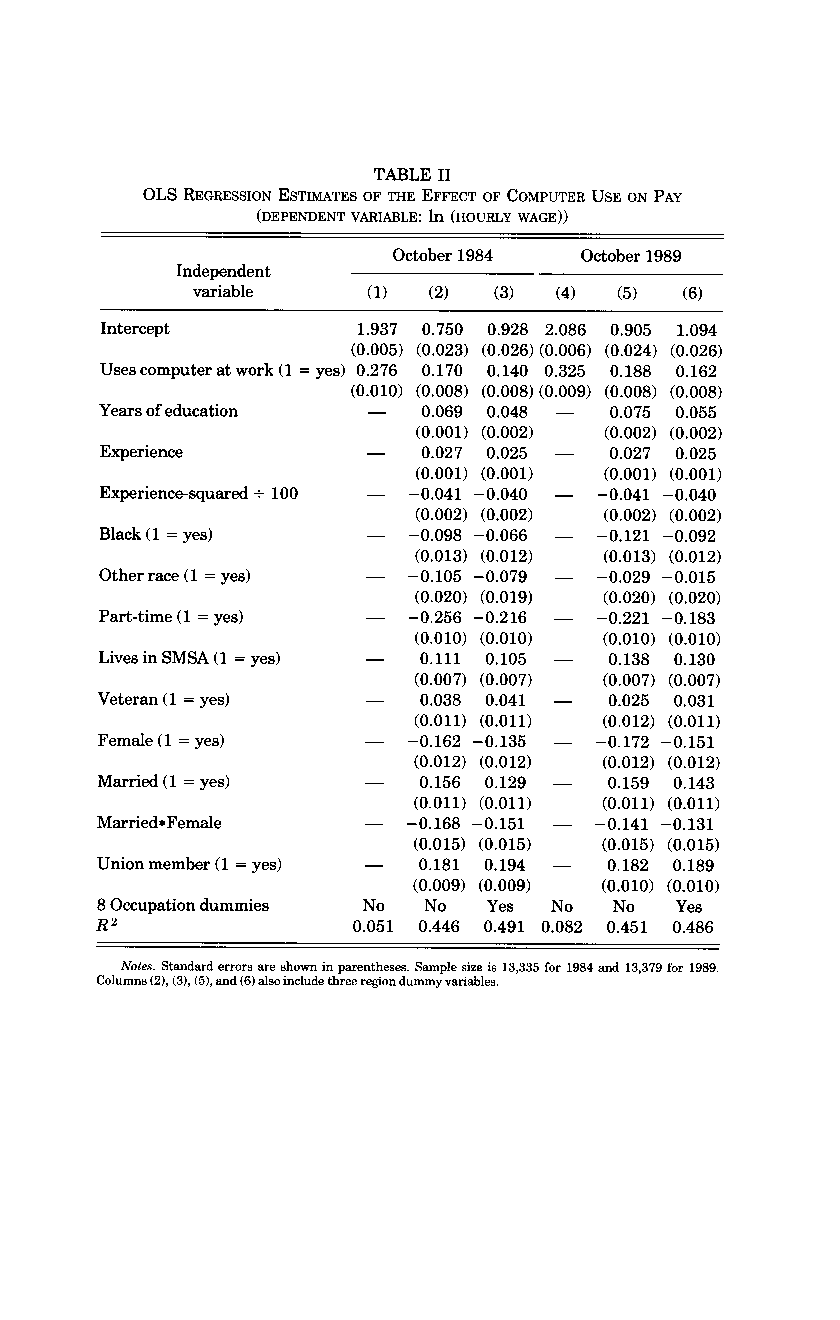
\includegraphics[width=0.7\linewidth]{graphs/kru_table2.pdf}
\end{figure}
\end{center}
 }

\begin{frame}
\frametitle{Robustness Checks}

   \begin{itemize}
     \item Coefficient gets smaller when other variables added
     \item Computer use at home and computer use at work.
     \item Narrow occupations: Secretaries $16\%$ of comp. users in 1984, and $77\%$ in 1989.
     \item Test Scores, Parental background from High school and beyond survey.
   \end{itemize}

\end{frame}

\frame{ \frametitle{}
\begin{center}
\begin{figure}[t]
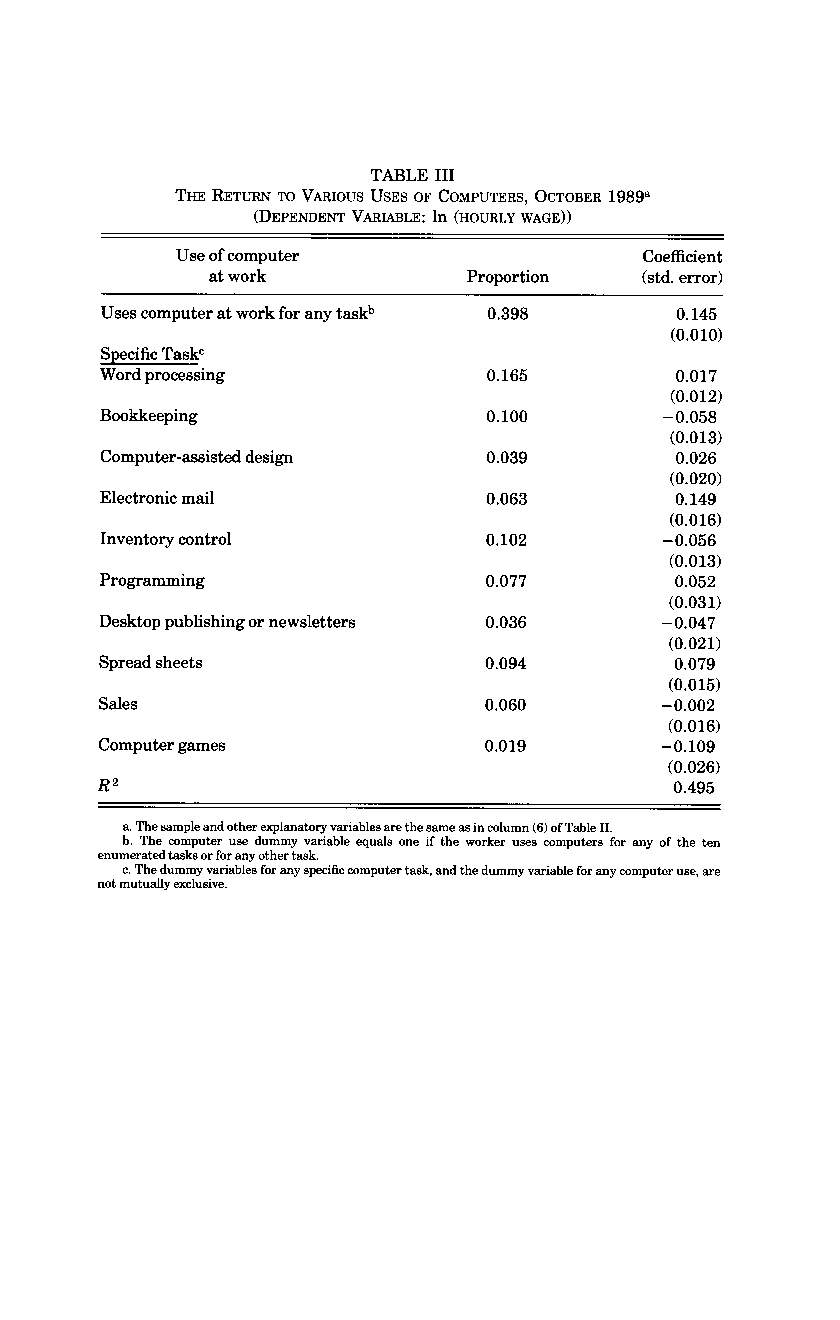
\includegraphics[width=0.9\linewidth]{graphs/kru_table3.pdf}
\end{figure}
\end{center}
 }


\frame{ \frametitle{}
\begin{center}
\begin{figure}[t]
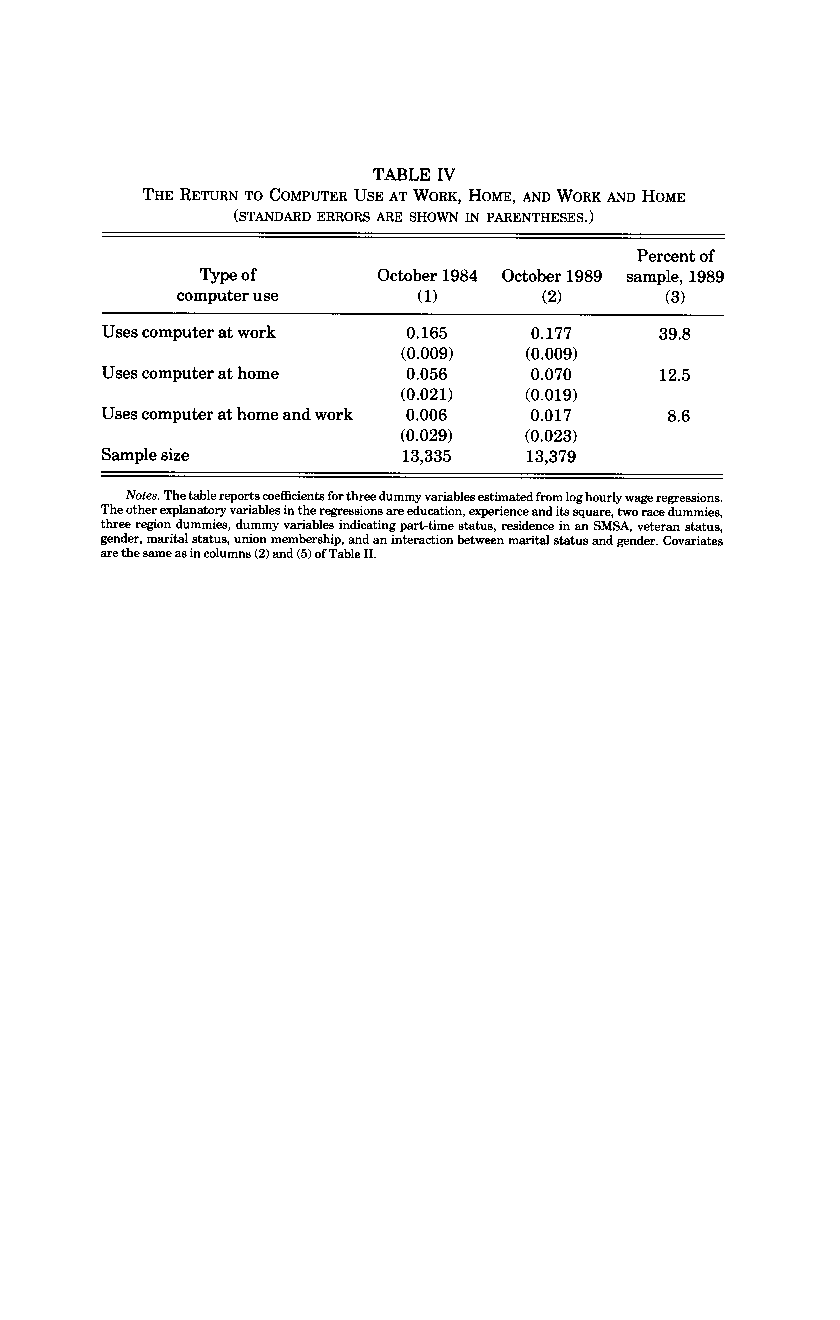
\includegraphics[width=0.9\linewidth]{graphs/kru_table4.pdf}
\end{figure}
\end{center}
 }


\frame{ \frametitle{}
\begin{center}
\begin{figure}[t]
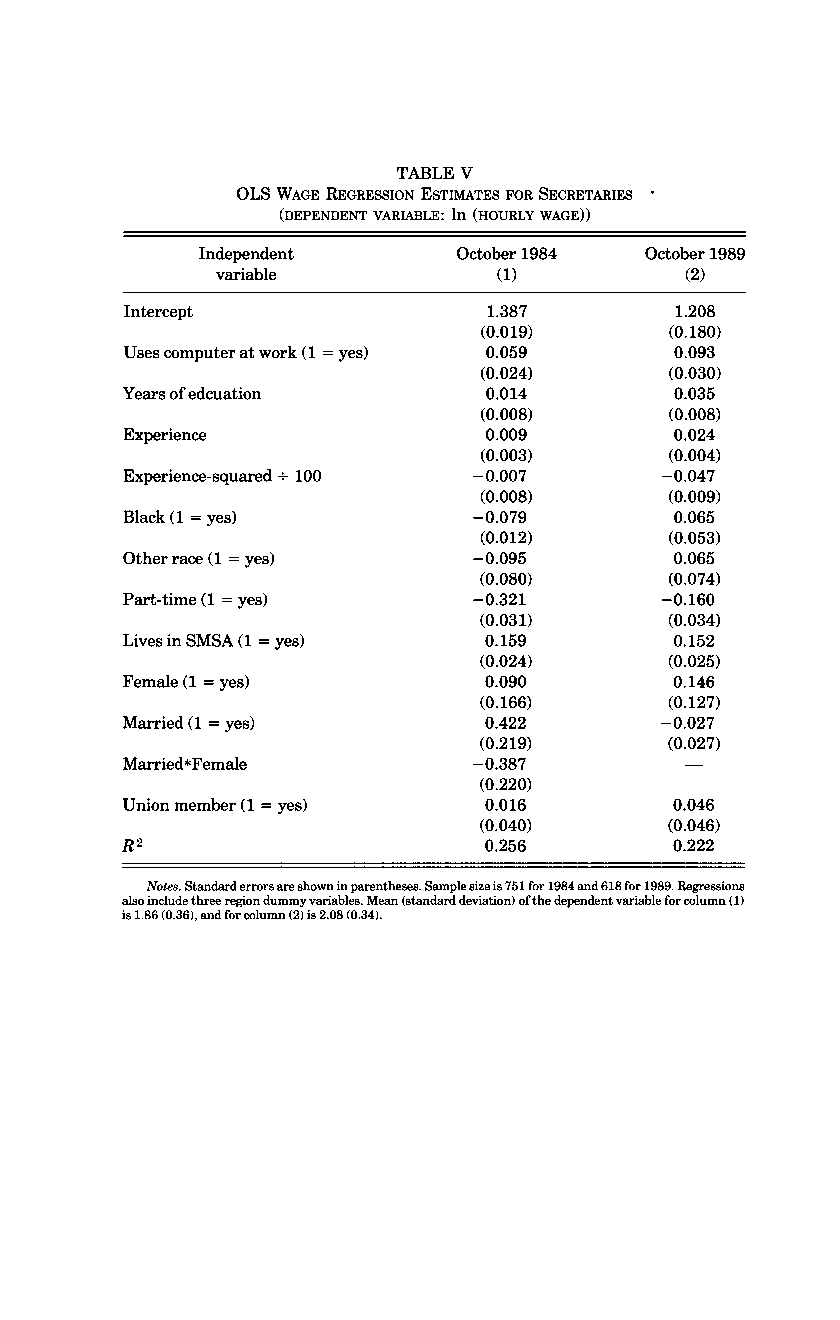
\includegraphics[width=0.8\linewidth]{graphs/kru_table5.pdf}
\end{figure}
\end{center}
 }

\frame{ \frametitle{}
\begin{center}
\begin{figure}[t]
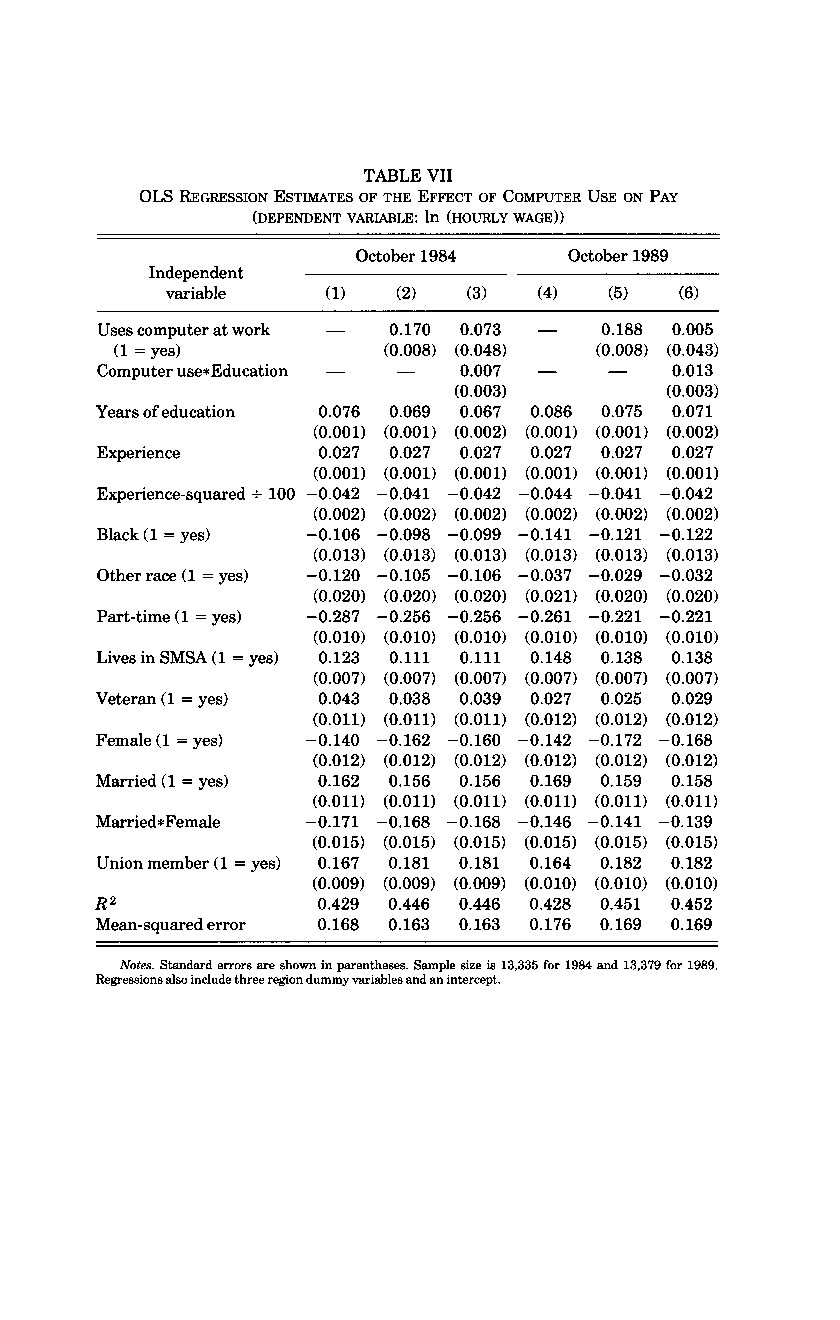
\includegraphics[width=0.8\linewidth]{graphs/kru_table7.pdf}
\end{figure}
\end{center}
 }



\begin{frame}
\frametitle{Returns to Computer Use Revisited}
 DiNardo and Pischke (2004):

     \begin{itemize} 
       \item German data, also cross section, but includes multitude of workplace tools i.e: office tools, hand tools etc.
       \item Qualification and Career Survey: 1985/86, 1991/92
       \item Check comparability of Germany vs. US
       \item Are the coefficients similar? External validity.
       \item What is the impact of other workplace tools on wages?
     \end{itemize}

\end{frame}

\frame{ \frametitle{}
\begin{center}
\begin{figure}[t]
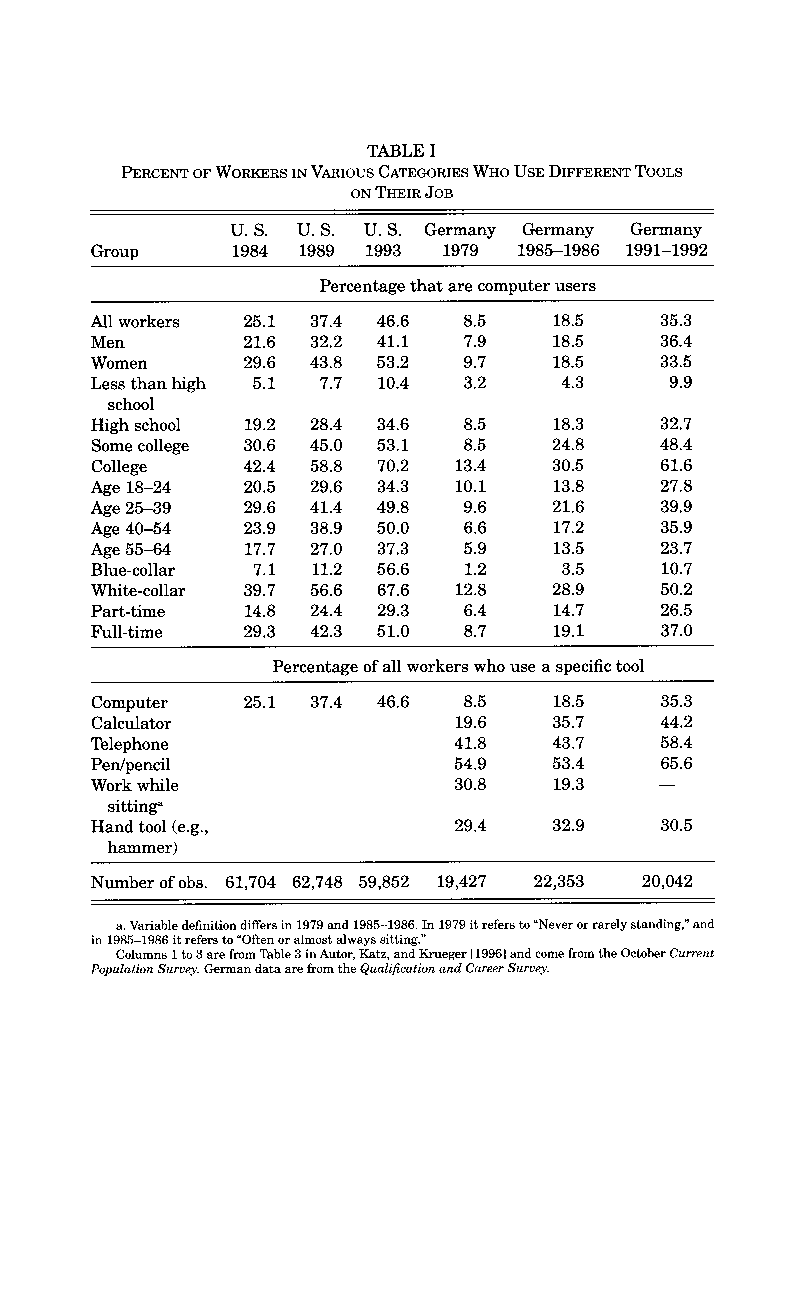
\includegraphics[width=0.6\linewidth]{graphs/pisc_table1.pdf}
\end{figure}
\end{center}
 }



\frame{ \frametitle{}
\begin{center}
\begin{figure}[t]
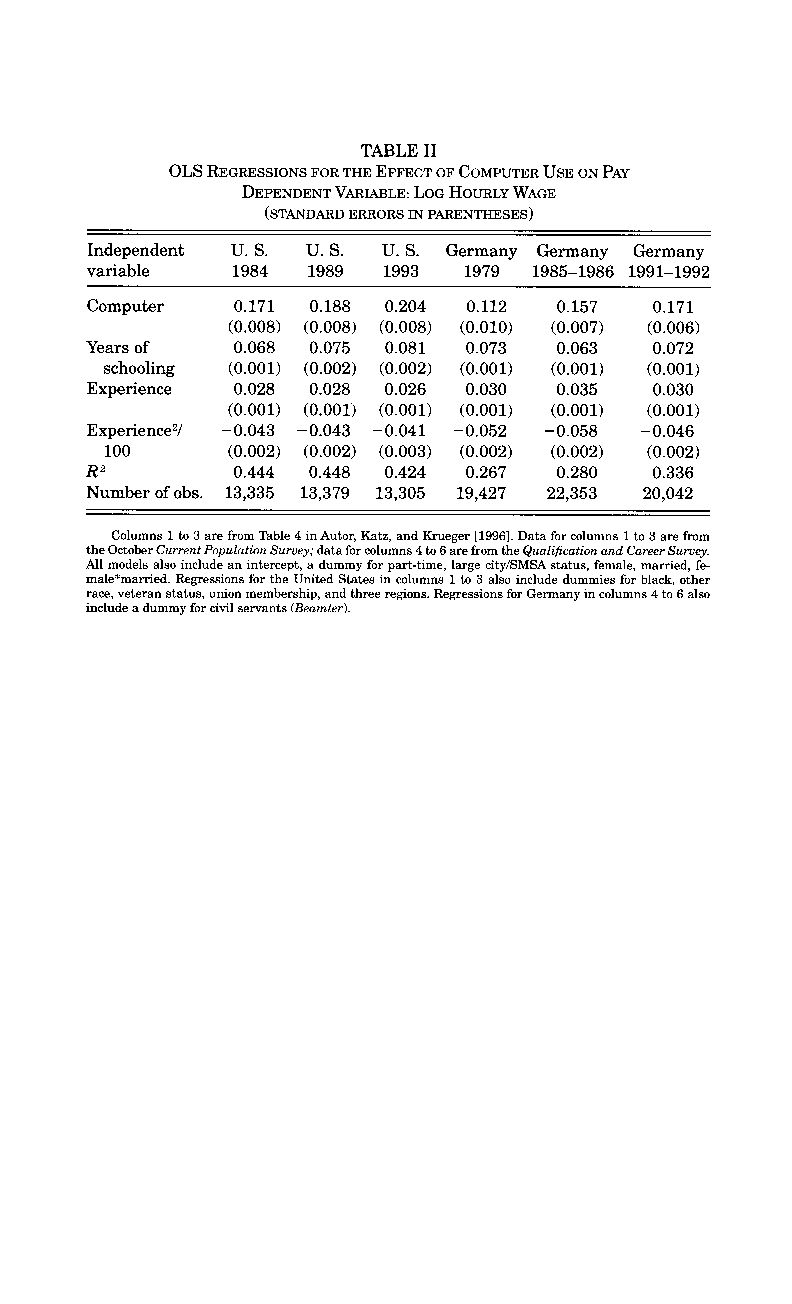
\includegraphics[width=1.0\linewidth]{graphs/pisc_table2.pdf}
\end{figure}
\end{center}
 }


\begin{frame}
\frametitle{Omitted Variable Bias}
\begin{itemize}
\item Table III
      \begin{itemize}
      \item Seperate regressions for each tool
      \end{itemize}
       \begin{eqnarray*}
           y_{i} &=& \beta_{0}+ \beta_{1}tool+\beta_{2}educ+...+u
      \end{eqnarray*}

\item Table III-b
      \begin{itemize}
      \item Enter tools together to check for correlation in use
      \end{itemize}
        \begin{eqnarray*}
             y_{i} &=& \beta_{0}+ \beta_{1}comp+\beta_{2}calc+\beta_{3}telep+...+u
        \end{eqnarray*}

\end{itemize}
\end{frame}

\frame{ \frametitle{}
\begin{center}
\begin{figure}[t]
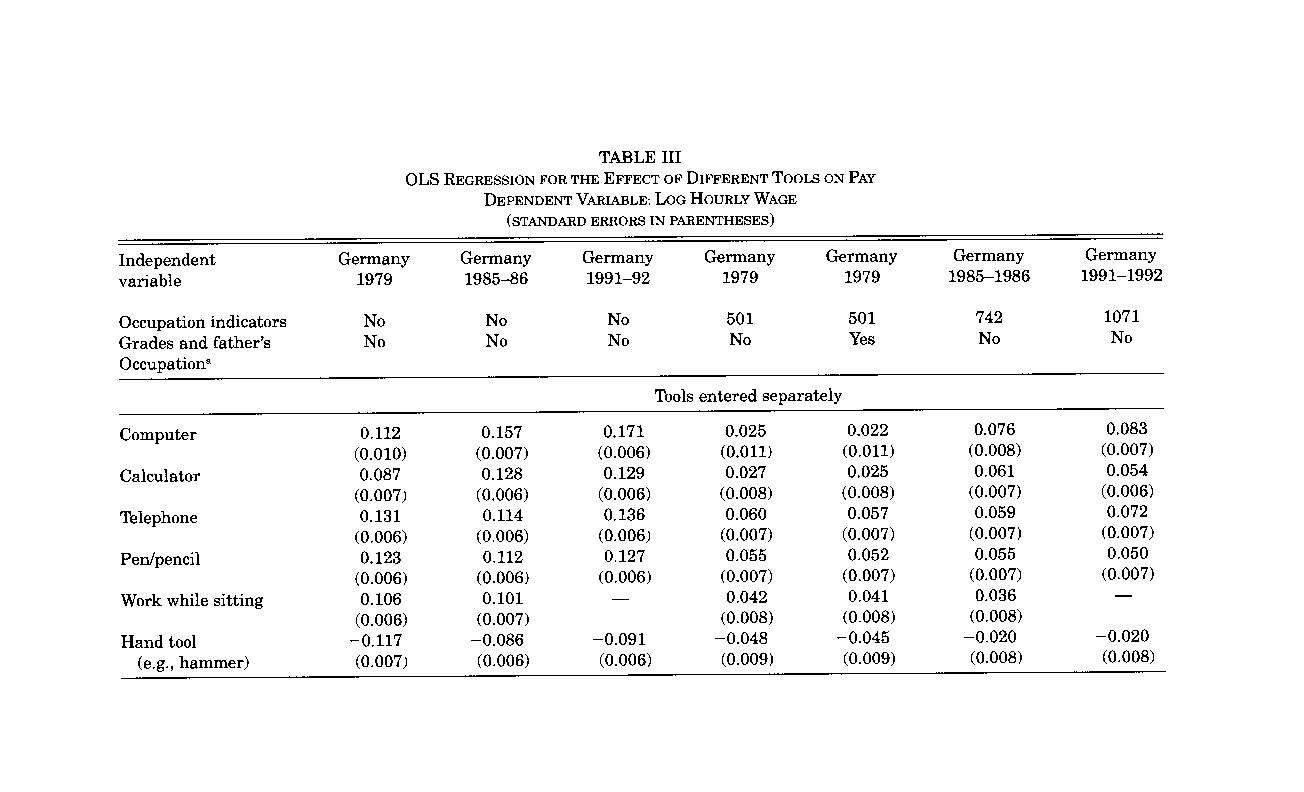
\includegraphics[width=1.0\linewidth]{graphs/pisc_table3.pdf}
\end{figure}
\end{center}
 }



\frame{ \frametitle{}
\begin{center}
\begin{figure}[t]
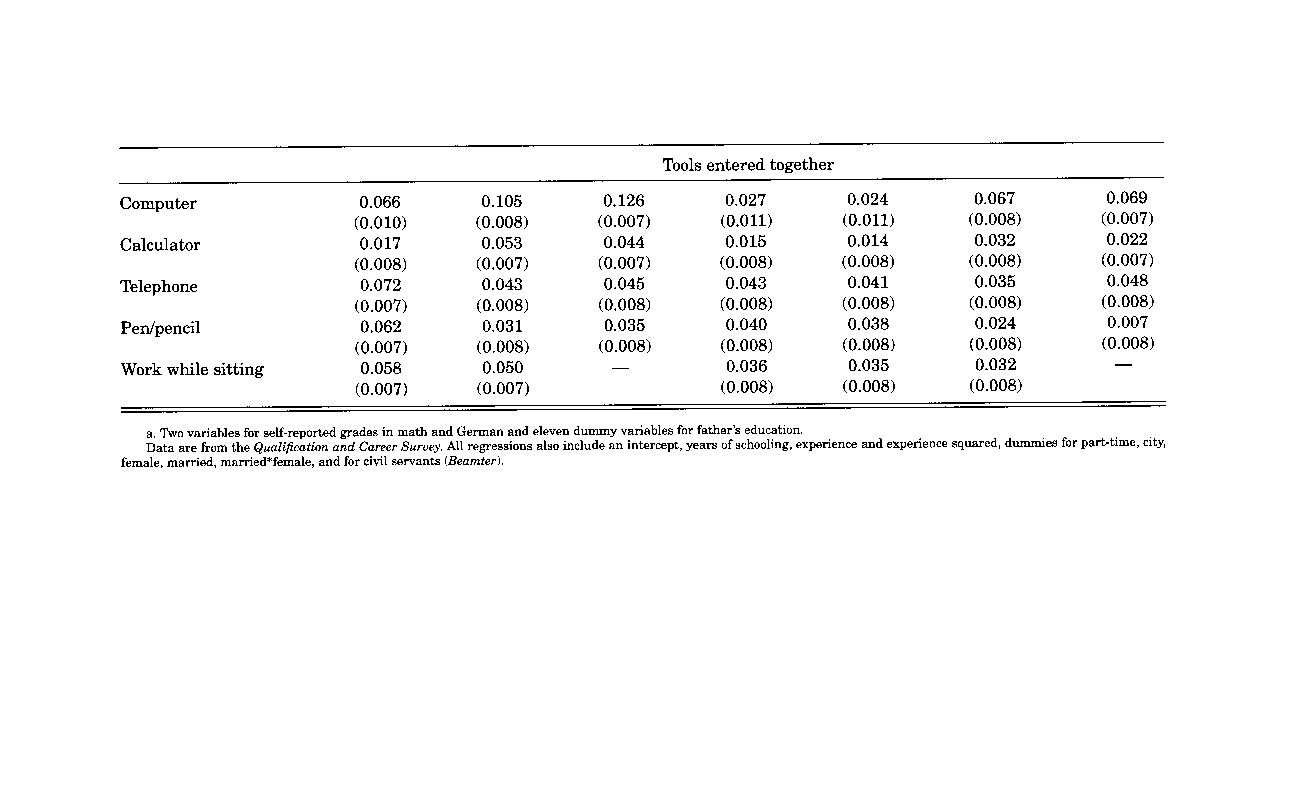
\includegraphics[width=1\linewidth]{graphs/pisc_table3b.pdf}
\end{figure}
\end{center}
 }

 \begin{frame}
\frametitle{Selection Problems}

     \begin{itemize} 
       \item What would be the ideal experiment?
       \item Randomly assign computers to workers?
       \item How are \emph{computer skills} awarded in the labor market?
       \item What about the \emph{skill} of using a pencil or a chair?
       \item Results point to substantial selection in who uses office tools
     \end{itemize}

\end{frame}
 


\end{document}
